\documentclass[12pt]{article}
\usepackage{fullpage}
\usepackage{amsmath}
\usepackage{graphicx}
\usepackage{enumerate}
\usepackage{float}
\usepackage{listings}
\usepackage{longtable}
\usepackage[table]{xcolor}
\usepackage{tabularx}
\usepackage{subfigure}
\usepackage{parskip}
\usepackage{bbm}
\usepackage[round]{natbib}
\restylefloat{figure}
\title{Gamifying the Transcriptome}
\author{Chidube Ezeozue and Joel Brooks}

\begin{document}
\bibliographystyle{apalike}
\renewcommand\refname{Bibliography}
\maketitle

\begin{abstract}

RNA-seq technology holds the potential for transcriptome assembly and abundance estimation from short reads of mRNA even in the presence of alternative splicing of transcripts. There are various computational methods such as Cufflinks \citep{trapnell2010transcript} for constructing the transcriptome from RNA-seq data, however, these algorithms rely on specific assumptions about the data and therefore ignore a large portion of the possible list of transcripts and their abundances that can explain relative exon abundances found by RNA-seq. Human-powered computation has previously been used to aid computational solutions for biological problems \citep{kawrykow2012phylo}. We extended the human computation idea to transcriptome assembly by
creating a block-based game that allow users to come up with transcripts that explain exon abundances for a gene without the requirement of any background knowledge of biology or computation. We used simulated data generated from the transcriptome for the mouse genome, and found that the human solutions found all the ground truth transcripts in many cases, and were able to find at least one of the original transcripts in most cases. We plan to host the game in a public location so that new solutions may be continuously submitted and possibly inspire future work with gamification or visualization of the transcript isoform problem.

\end{abstract}

\section*{Background}
Alternative splicing is an important functional occurrence in eukaryotes \citep{pan2008deep}. These splicing events allow a single gene to produce multiple mRNA transcripts and thus increases biological complexity, as different isoforms (different mRNA transcripts from the same gene) may be translated to different proteins or induce a different regulation of the same protein \citep{trapnell2010transcript}. These events are quite common, and evidence suggests they occur in roughly 95\% of multiexonic human genes.

The development of RNA-seq technology has greatly advanced the possibility of mRNA transcript assembly, but detecting isoforms from the millions of short reads generated by RNA-seq is a computationally daunting problem because the reads are too short to span an entire mRNA transcript. Existing methods are able to asses relative exon abundance for a gene from RNA-seq data with relatively high accuracy \citep{trapnell2009tophat}. However, reconstructing the set of mRNA isoforms that produced those exon abundances is a computationally complex problem. One notable example of methods that attempted to do this, Cufflinks, uses weighted bipartite graphs to find the minimum set of transcripts that explain the set of reads \citep{trapnell2010transcript}. Another method, Scripture, constructs ``connectivity graphs" from spliced and unspliced reads. The method then suggests isoform transcripts based on alternative paths through the graphs as well as statistics obtained from a sliding window through the genome \citep{guttman2010ab}. Optimization-based approaches have also been explored by tools like IsoLasso. These techniques frame the problem as an optimization subject to minimizing the number of transcripts found and maximizing the agreement with read data and expression levels \citep{li2011isolasso}.

In this project, we explored the possibility of humans finding alternative sets of transcripts through a game-based interface. Human-powered computation has previously been shown to be of use in biological problems \citep{kawrykow2012phylo, cooper2010predicting}. For example, Phylo allowed humans with no understanding of biology to perform multiple sequence alignment (MSA). Phylo was designed to abstract the underlying biology away by representing nucleotide bases as colored blocks.  The intuition behind such an abstraction is that humans are good at visual pattern recognition. Using Phylo, humans were indeed able to outperform state of the art MSA algorithms for certain sequences. We used a similar motivation to explore the idea of humans reconstructing transcript isoforms from relative abundances of exons by conveying the problem in a simple block-based puzzle. This makes it possible for a person with no understanding of computational biology to play and find potentially useful solutions. The human solutions were then scored using a formula we developed aided by the ground truth present in simulated read data. 

\section*{Methods}

\subsection*{Game overview}
The game is designed to utilize human-powered computation to explore transcriptome possibilities for certain genes using experimental data from
RNA-seq. Experimental data is first mapped to a genome using a splicing-aware read aligner such as TopHat \citep{trapnell2009tophat}. From these mappings,
relative abundance levels of each exon within a gene are inferred.

When the user first starts the game, they are presented with a puzzle as shown in Figure \ref{fig:gamescreen}. This puzzle represents
the relative abundance of exons within a gene. A player must clear all the blocks in each column in order to complete the puzzle. Users accomplish this by 
creating and adding transcripts to their list. Single-colored blocks represent the abundance of reads mapped to just one exon so they can be removed by any 
transcript that includes that exon. However, blocks with two colors represent the abundance of reads that were mapped to more than one exon. These ``linked"
blocks are removed when \emph{both} exons that the reads were mapped to are selected, however, no exons can be selected in between the ``linked" blocks as
we assume a read can only map to more than one exon if those two exons appear contiguously within a transcript. For example, in the puzzle shown in Figure \ref{fig:gamescreen}, the ``linked" blocks in columns 4 and 8 can only be removed by the addition of a transcript that has those columns but doesn't include columns 5-7. Taking these rules into consideration, the user
tries to build a transcript list that removes all of the blocks in the puzzle and achieves a maximal score. After completion of a puzzle, the user's score for that puzzle is
sent back to the server and stored in the database. The user then has the option to continue the game with a new puzzle.

\begin{figure}[H]
\centering
\subfigure[Screenshot of Puzzle]{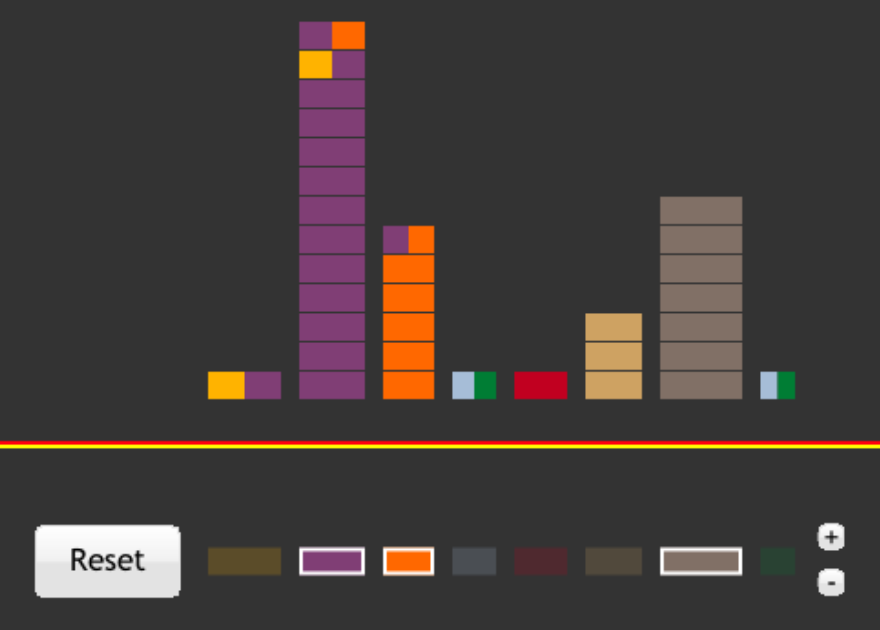
\includegraphics [width=0.45\textwidth]{puzzleshot.png}} 
\subfigure[List of Transcripts Created]{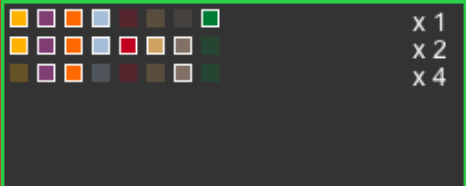
\includegraphics [width=0.45\textwidth]{listshot.png}} 
\caption{Game Screenshot}\label{fig:gamescreen}
\end{figure}

\subsection*{Data acquisition and preparation}
We simulated short reads using Flux Simulator \citep{sammeth2010flux} running on data from the mouse mm9 genome annotated with the locations of genes, exons, and transcripts. To make the problem more tractable, we eliminated all instances of intron-skipping and used only genes with at least two known transcripts. We also only included genes where the known transcripts differed by the presence or absence of exons i.e. we ignored the phenomena of varying transcription starts and represented the data such that all transcripts are assumed to start at the same base in the start exon(s). We also ignored polyadenylation sites. 

We simulated over 6 million reads of 75 nucleotides long each from 7,901 transcripts of 3324 genes (average transcripts per gene = 2.4) and pushed information about read count and mapped exons to the database. Since the simulator created random expression levels for each transcript provided leading to the possibility that some transcripts may not have been expressed, we only included in the puzzle genes with at least 2 expressed transcripts.

Since the number of reads mapped to an exon depends heavily on the length of the exon, we normalized the read counts by exon length. Additionally, we also scaled the read counts to be able to fit most puzzles on typical computer screens. If $r_i$ and $r_{ij}$ are the original read counts for reads falling wholly in one exon $e_i$ and reads falling across exons $e_i$ and $e_j$ respectively, and $k$ is the read length, the normalized counts,  $r'_i$ and $r'_{ij}$, and scaled counts, $r''_i$ and $r''_{ij}$, are obtained by:
\begin{align*}
r'_i &= \frac{r_i}{|e_i|} \\
r'_{ij} &= \frac{r_{ij}}{2k} \\
r''_i &= \frac{r'_i}{\underset{r*' \in r', r*' \not = 0}{min(r*')}} \\
r''_{ij} &= \frac{r''_{ij}}{\underset{r*' \in r', r*' \not = 0}{min(r*')}} \\
\end{align*}

\subsection*{Game implementation}
The game interface was built using the LimeJS (http://www.limejs.com/) HTML5 game framework . This framework provides methods for creating shapes,
animations, and handling user interaction events. It allowed us to focus more on developing the core functionality of the game.
Additionally, the fact that the game is implemented in HTML5 and Javascript means that it can be played in most popular browsers running on both desktop and mobile hardware.

We also made use of Kenneth Kelly's list of 22 colors of maximum contrast \citep{green2010colour}. This allowed us to assign each exon in a particular puzzle a unique color that was easily distinguishable from the colors of all the other exons. This enabled us to present genes to 
users in a manner that was both visually appealing and functional.

We utilized a Python/Django server for communicating with the frontend using the Javascript Object Notation (JSON) format. The database used is a MySQL database running on the internal CSAIL MySQL servers. 

The game is currently hosted at http://chameleon.csail.mit.edu:3000/transcriptomeapp/ and will be available for play at that location until December 31st.

\subsection*{Solution scoring} 

\subsubsection*{Frontend}
\label{sec:scoring}
Since there will be no ground truth for real, unsimulated data, it is essential for us to have
a scoring system that is both able to influence user's approach to finding accurate lists of transcripts for a particular gene as well as to be independent of existing transcript annotations. We hypothesize that the best results will be small lists of unique transcripts, transcripts that include more exons, and transcripts that include more nucleotide bases.
Thus we developed the following scoring metric for scoring transcript list $T$ :
\begin{equation*}
S(T) = d(T) * \sum_{i=1}^{|T|} \log{|T_i|} * \sum_{k = 1}^{|T_i|} \log{n_{ik}}
\end{equation*}
\begin{equation*}
d(T) = \frac{1}{1+e^{\gamma |T|}}
\end{equation*}
where $|T|$ is the number of transcripts in $T$, $|T_i|$ is the number of exons in transcript $T_i$, and $n_{ik}$ is the number of bases in exon $k$ of transcript $i$.
$d$ is a discount factor with parameter $\gamma$ that controls how longer lists of transcripts are devalued. Setting $\gamma = .001$ seemed to achieve the desired
discounting of long transcript lists within the context of the game. Furthermore, the $\log{|T_i|}$ factor ensures that transcripts that only contain one exon will not factor
into the player's score, which is a desirable property given that players often have to add transcripts with one exon in order to finish out a puzzle.
\subsubsection*{Backend}
In addition to computing the precision and recall, we also scored a puzzle using the expression levels of the transcripts found against the expression levels in the ground truth. Given $T'$, the set of transcripts in the ground truth of a particular gene/puzzle, and $e(T'_i)$ and $e(T_i)$, the relative expression levels of the transcripts in the ground truth and user solution, respectively, the score, $S_{truth}(T_i)$, for a particular transcript is computed as:
\begin{align*}
S_{truth}(T_i) &= \sum\limits_{j = 1}^{|T'|}(1 - abs(e(T'_j) - e(T_i)))\mathbbm{1}\{T'_j = T_i\} \quad \text{where $\mathbbm{1}\{\}$ is an indicator function}
\end{align*}
The score for the entire puzzle $S_{truth}(T)$ is then given by:
\begin{align*}
S_{truth}(T) = \frac{\sum\limits_{i=1}^{|T|} S_{truth}(T_i)}{max(|T'|, |T|)}
\end{align*}
This gives a score of 1 for solutions with perfect transcript and expression level identification, a score of 0 for solutions where no transcript is perfectly identified and a score between 0 and 1 for solutions with some error in transcript identification or expression level assignment.

\section*{Results and Discussion}
In just over 66 hours of making the game available to players, we received close to 250 submissions and made some interesting preliminary observations. Most of the user results discovered at least one of the transcripts underlying the read data and almost a third of the user results discovered all the transcripts as shown in the recall plot in Figure \ref{fig:precisionandrecall}. Figure \ref{fig:precisionandrecall} also shows that most of the solutions also had at least one accurate transcript and a few were entirely accurate. This suggests that the game representation was helpful in guiding the players to discover the transcripts. It is interesting to note that most of the 2-exon gene transcripts were fully discovered. However, the precision and recall is reduced as the number of exons increase. It is also interesting to note that the difference between recall and precision suggests that users, in general, seemed to find too many transcripts, and thus a frontend scoring scheme that penalizes longer lists of transcripts more may produce lead to better results.

Some of the results, however, did not discover any of the correct transcripts and had zero precision. There are two possible reasons for this: it is possible that there were players who did not pay enough attention to the game to obtain good results; it is also possible that some puzzles were particularly difficult. As a future direction, it will be useful to track some identifier for every user and use their average performance on multiple puzzles to weight our confidence in their submissions. As more users play each puzzles, it will also become possible to identify puzzles that are particularly difficult as well as identifying outlier puzzle solutions.

\begin{figure}[H]
\centering
\subfigure[Precision]{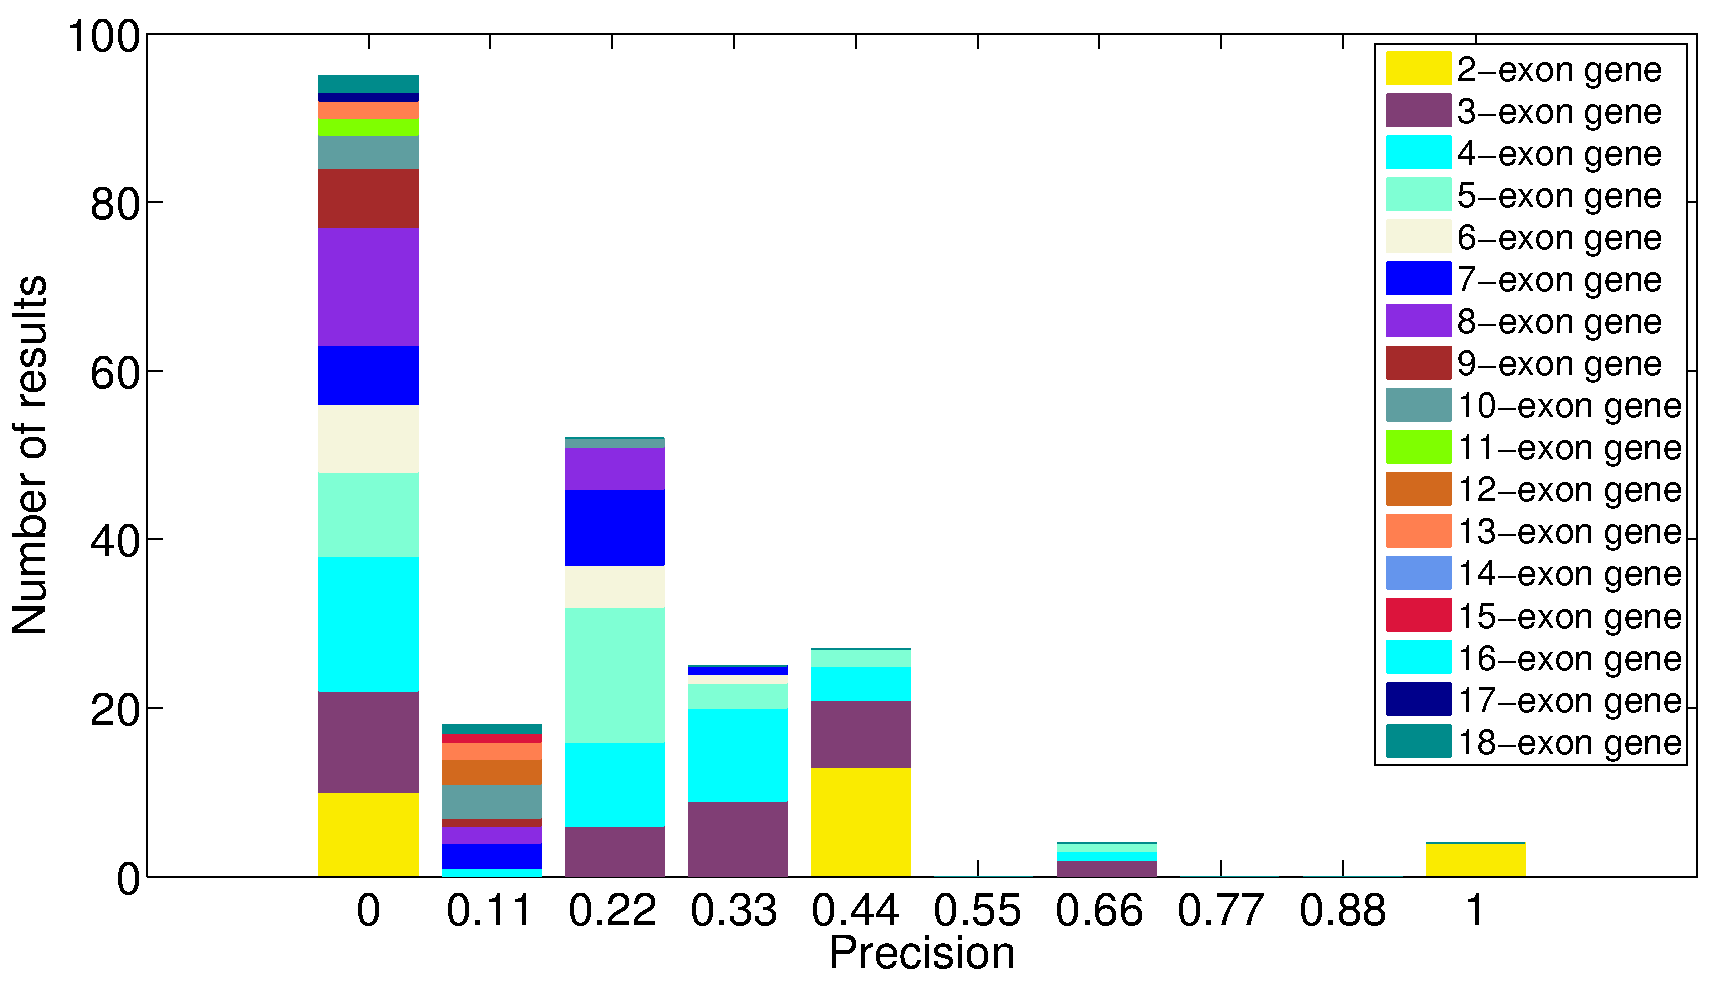
\includegraphics [width=0.45\textwidth]{Precision}} 
\subfigure[Recall]{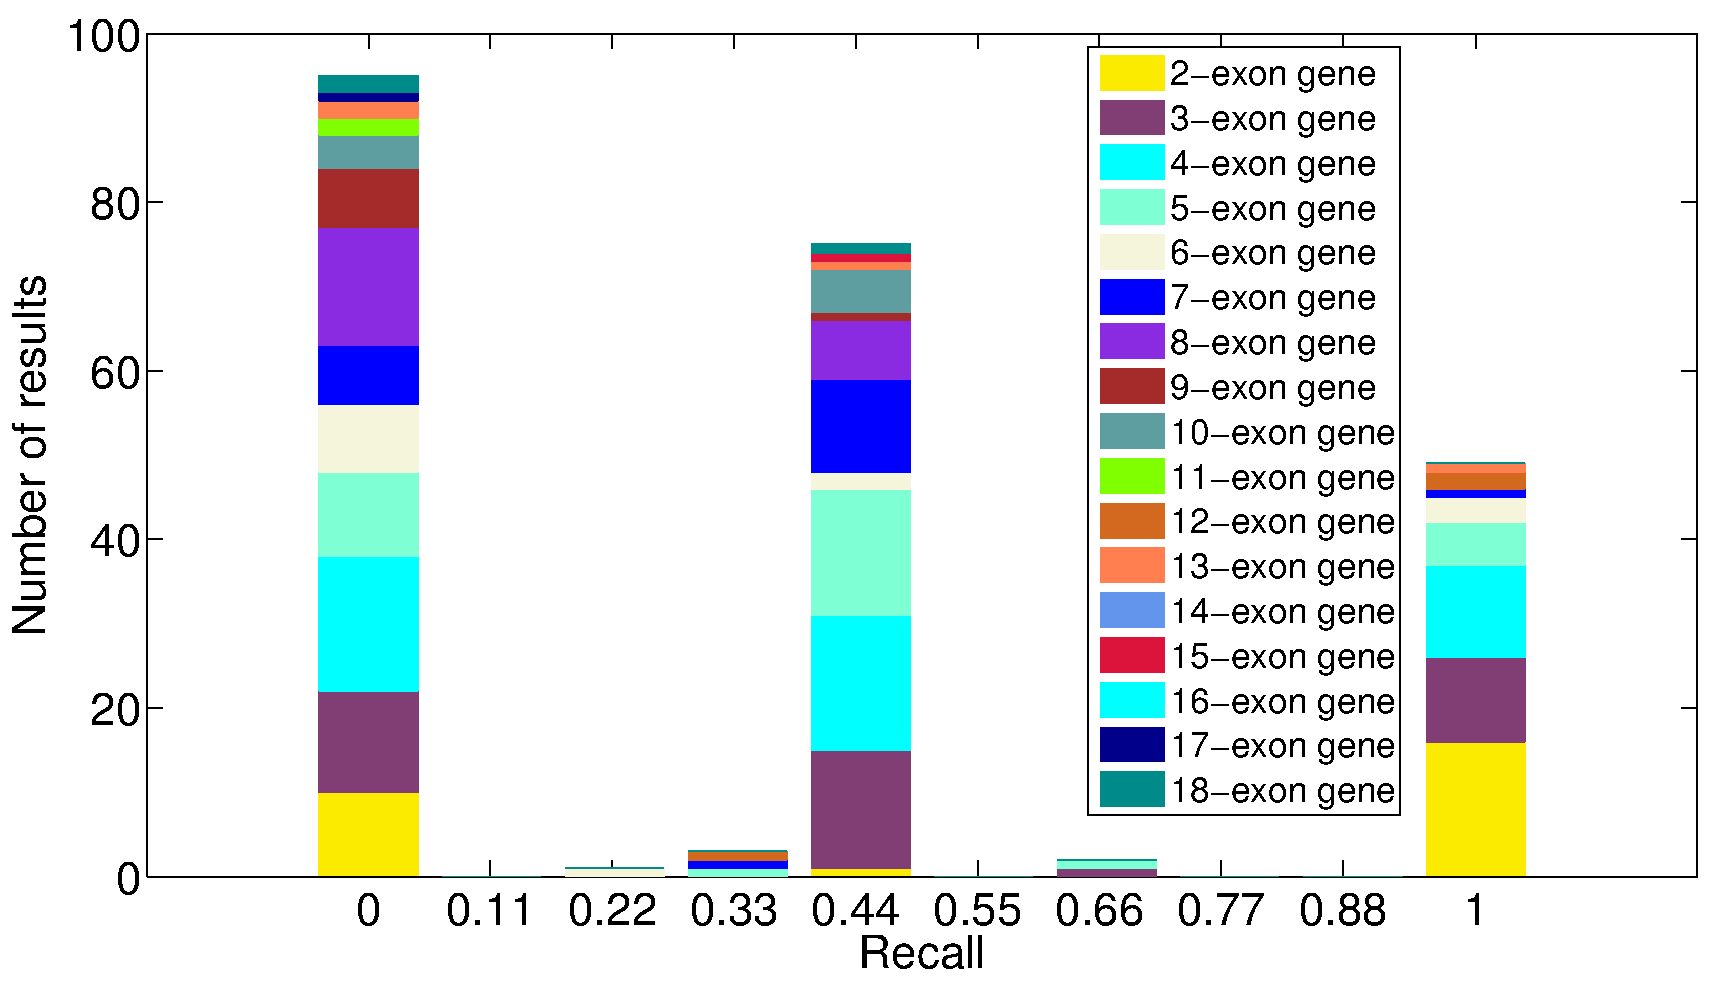
\includegraphics [width=0.45\textwidth]{Recall}} 
\caption{Precison and Recall of user-submitted results}\label{fig:precisionandrecall}
\end{figure}

In the \emph{Solution scoring} section, we described a frontend scoring scheme utilizing specifics of a solution and a backend scoring scheme against the ground truth. It is our intention to manually or automatically learn the frontend scoring scheme for use against actual, unsimulated data with no ground truth. Figure \ref{fig:score} shows that, despite encouraging results in detecting transcripts, players have difficulty in correctly assigning expression levels. The plots also demonstrate a disconnect between the front-end scores and backend ground truth-based scoring. This indicates the need for further work in fine-tuning the frontend scoring scheme to correlate more closely with the performance against ground truth while allowing players find novel transcripts that are not
identified by existing computational methods. Additionally, we believe that it is possible to apply machine learning algorithms to the frontend scoring parameters and learn the optimal scoring parameters.

\begin{figure}[H]
\centering
\subfigure[Expression Accuracy]{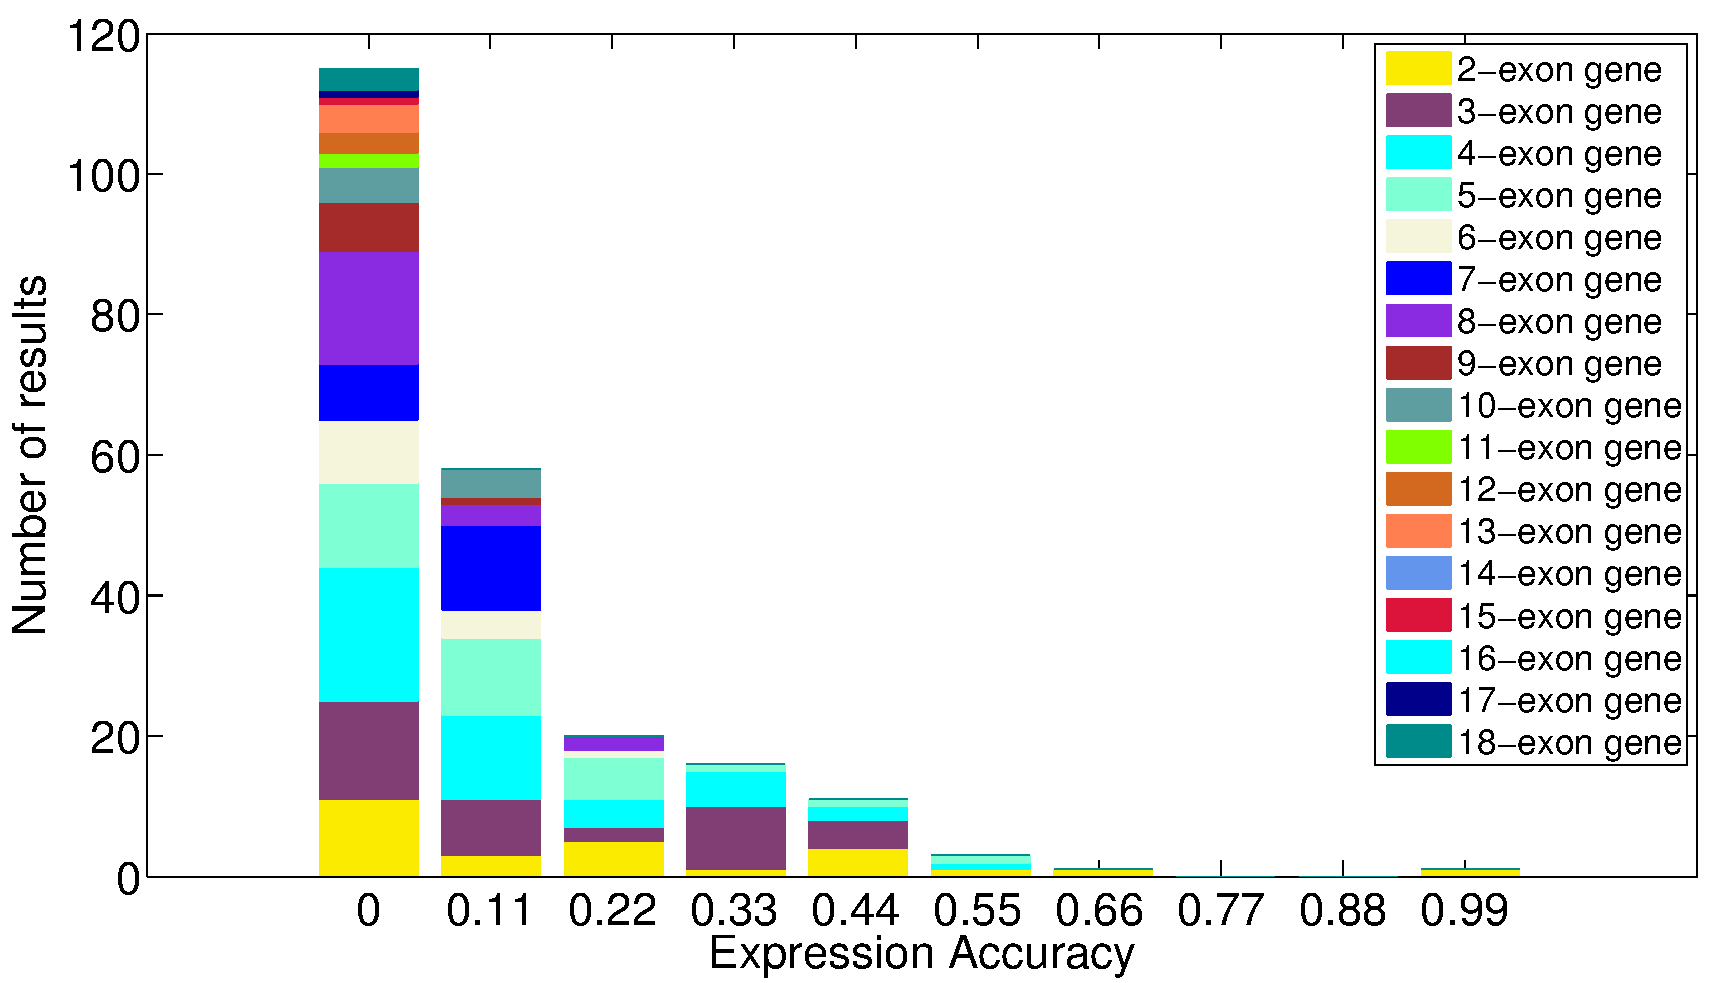
\includegraphics [width=0.45\textwidth]{ExpressionAccuracy}}
\subfigure[Frontend Score]{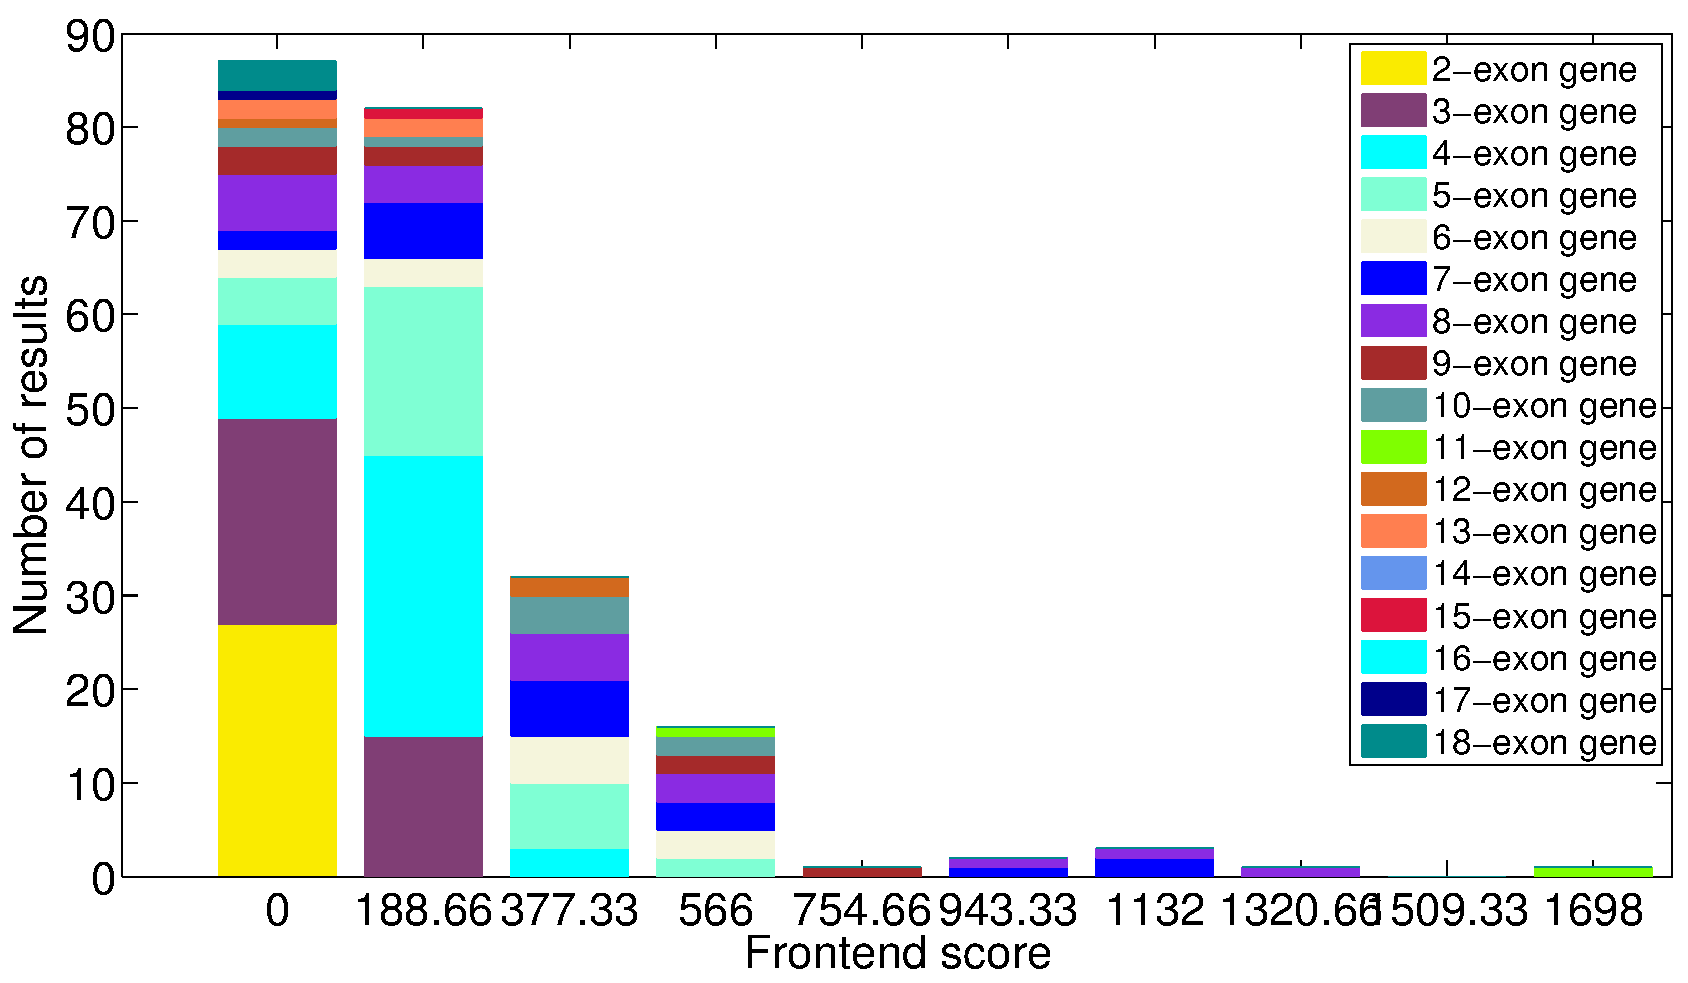
\includegraphics [width=0.45\textwidth]{FrontendScore}}
\caption{Expression Accuracy and Frontend Score of user-submitted results}\label{fig:score}
\end{figure}

An unanticipated outcome of this game is that we realize that, in addition to allowing users recreate the transcriptome, we had also created a visualization tool that could give scientists an interesting view into the transcriptome. Visualization remains an important step in the research process and this tool is a first step towards another way of looking at how genes are spliced.

\section*{Future goals}

We originally planned to have users play puzzles that were generated from real RNA-seq data in addition to the synthetic data generated using Flux Simulator.
We obtained the same experimental RNA-seq data used by Trapnell et al. in the original Cufflinks paper \citep{trapnell2010transcript}. We mapped the reads to 
the mouse genome using TopHat, and were hoping to construct puzzles based on these data in the same manner as we did with the synthetic data. However, due
to time constraints, we felt it was better to focus primarily on the synthetic data, as this allowed us to compare user solutions to a ground truth transcriptome. We also attempted to compare our results with existing algorithms like Cufflinks, Scripture and IsoLasso. Due to time constraints and issues with file formats we were unable to complete these comparisons.

We recruited volunteer testers for our game from the MIT community: friends, classmates, dorm mates etc. and received qualitative feedback on the likeability of the game and the learning curve in addition to discovering transcripts and expression levels. We received mostly
positive feedback from the users that played the game, however, a significant amount of people found the rules of the game to be somewhat confusing. In response,
we would like to make the rules regarding ``linked" blocks removal clearer. The confusion was probably due to lack of specific examples of how the ``linked" blocks
work. Thus, adding a tutorial level, gameplay video, or even screenshots that focus on this specific aspect of gameplay would likely help to clear up the confusion. In future versions, we will also stratify the game by difficulty levels and allow players gain experience at simpler levels before moving on to more difficult puzzles. 

Another aspect of the game that we would like to explore is the effect of the within game scoring metric on user solutions. As one user review pointed out, we could incentivize users to do better by providing a ranking of their scores against other players. Due to time constraints and limited puzzle coverage by multiple players, we were unable to include this
feature as part of the game.

\section*{Comparison with original proposal}

Our main goal from the beginning of the project was to implement the game, and we were able to create a fully functionally final product and test its viability on a select set of users. The main
difference between our original proposal and our final set of accomplishments is the level of detail to which the user results were analyzed. We originally wanted to run a pool of algorithms
on the same data that we used to construct the puzzles used in the game, however, we were not able to accomplish this due to time constraints. This became more apparent when we
completed midcourse report and analyzed what we had left to accomplish. However, we feel that the
algorithmic analysis, while potentially very beneficially, is secondary to the creation and demonstration of the game. Thus, even though we did not achieve all that we had originally set out to accomplish, we are elated at the level of success we achieved.

\section*{Commentary on experience}

In general, starting our tasks earlier would have allowed us to better manage time and possibly achieve more of the goals we set out to accomplish in our original project proposal.
There were unanticipated delays that could have been mitigated by leaving more time margins than we thought we needed. For example, data collection was not an issue for us, but
setting up the simulator and analyzing the results was not as trivial as it first seemed. Additionally, there are always unforeseen roadblocks in coding heavy projects, and this project
required a significant amount of design and programming. Identifying these bottlenecks earlier could have helped us manage them better.

One of the great things about working on this project is that we have a finished tool that we can  send out to the general public and have people try out. We received quite a bit of feedback from the initial users and people generally had positive things to say. We are proud to be able to apply the things we learnt in class to a tool that can be appreciated by people that previously knew nothing about computational biology.

\section*{Commentary on peer review process}

The reviews were helpful because they all pointed out that our original timeline was not granular enough and needed to be broken down. We incorporated an updated timeline in our midcourse
report, which was important as it made us step back and analyze how far we had come from when we started the project, and what we had left to do in the time that remained. Breaking down lumped-up steps in the original timeline also allowed us identify bottlenecks that would have been critical in the course of the project. This
allowed us to better prioritize the items that remained on our agenda, and helped us set a clear path to our project completion. The only other consensus item from the reviews were general
concerns about the playability of the game, however, we felt these points were not really actionable outside of what we were already aiming to accomplish.

\section*{Division of labor}

Chidube performed the simulations on synthetic data, developed and managed the web server and data processing utilities, and performed the post collection data analysis and server-side scoring. Joel prepared the experimental RNA-seq data, designed the web browser interface, and was the primary developer of the game functionality and frontend scoring system. Both Chidube and Joel contributed to high level game and project design, as well as writing of the proposals and final report.

\bibliography{frbib}

\end{document}
